% Options for packages loaded elsewhere
\PassOptionsToPackage{unicode}{hyperref}
\PassOptionsToPackage{hyphens}{url}
\PassOptionsToPackage{dvipsnames,svgnames,x11names}{xcolor}
%
\documentclass[
  letterpaper,
  DIV=11,
  numbers=noendperiod]{scrartcl}

\usepackage{amsmath,amssymb}
\usepackage{iftex}
\ifPDFTeX
  \usepackage[T1]{fontenc}
  \usepackage[utf8]{inputenc}
  \usepackage{textcomp} % provide euro and other symbols
\else % if luatex or xetex
  \usepackage{unicode-math}
  \defaultfontfeatures{Scale=MatchLowercase}
  \defaultfontfeatures[\rmfamily]{Ligatures=TeX,Scale=1}
\fi
\usepackage{lmodern}
\ifPDFTeX\else  
    % xetex/luatex font selection
\fi
% Use upquote if available, for straight quotes in verbatim environments
\IfFileExists{upquote.sty}{\usepackage{upquote}}{}
\IfFileExists{microtype.sty}{% use microtype if available
  \usepackage[]{microtype}
  \UseMicrotypeSet[protrusion]{basicmath} % disable protrusion for tt fonts
}{}
\makeatletter
\@ifundefined{KOMAClassName}{% if non-KOMA class
  \IfFileExists{parskip.sty}{%
    \usepackage{parskip}
  }{% else
    \setlength{\parindent}{0pt}
    \setlength{\parskip}{6pt plus 2pt minus 1pt}}
}{% if KOMA class
  \KOMAoptions{parskip=half}}
\makeatother
\usepackage{xcolor}
\setlength{\emergencystretch}{3em} % prevent overfull lines
\setcounter{secnumdepth}{-\maxdimen} % remove section numbering
% Make \paragraph and \subparagraph free-standing
\makeatletter
\ifx\paragraph\undefined\else
  \let\oldparagraph\paragraph
  \renewcommand{\paragraph}{
    \@ifstar
      \xxxParagraphStar
      \xxxParagraphNoStar
  }
  \newcommand{\xxxParagraphStar}[1]{\oldparagraph*{#1}\mbox{}}
  \newcommand{\xxxParagraphNoStar}[1]{\oldparagraph{#1}\mbox{}}
\fi
\ifx\subparagraph\undefined\else
  \let\oldsubparagraph\subparagraph
  \renewcommand{\subparagraph}{
    \@ifstar
      \xxxSubParagraphStar
      \xxxSubParagraphNoStar
  }
  \newcommand{\xxxSubParagraphStar}[1]{\oldsubparagraph*{#1}\mbox{}}
  \newcommand{\xxxSubParagraphNoStar}[1]{\oldsubparagraph{#1}\mbox{}}
\fi
\makeatother

\usepackage{color}
\usepackage{fancyvrb}
\newcommand{\VerbBar}{|}
\newcommand{\VERB}{\Verb[commandchars=\\\{\}]}
\DefineVerbatimEnvironment{Highlighting}{Verbatim}{commandchars=\\\{\}}
% Add ',fontsize=\small' for more characters per line
\usepackage{framed}
\definecolor{shadecolor}{RGB}{241,243,245}
\newenvironment{Shaded}{\begin{snugshade}}{\end{snugshade}}
\newcommand{\AlertTok}[1]{\textcolor[rgb]{0.68,0.00,0.00}{#1}}
\newcommand{\AnnotationTok}[1]{\textcolor[rgb]{0.37,0.37,0.37}{#1}}
\newcommand{\AttributeTok}[1]{\textcolor[rgb]{0.40,0.45,0.13}{#1}}
\newcommand{\BaseNTok}[1]{\textcolor[rgb]{0.68,0.00,0.00}{#1}}
\newcommand{\BuiltInTok}[1]{\textcolor[rgb]{0.00,0.23,0.31}{#1}}
\newcommand{\CharTok}[1]{\textcolor[rgb]{0.13,0.47,0.30}{#1}}
\newcommand{\CommentTok}[1]{\textcolor[rgb]{0.37,0.37,0.37}{#1}}
\newcommand{\CommentVarTok}[1]{\textcolor[rgb]{0.37,0.37,0.37}{\textit{#1}}}
\newcommand{\ConstantTok}[1]{\textcolor[rgb]{0.56,0.35,0.01}{#1}}
\newcommand{\ControlFlowTok}[1]{\textcolor[rgb]{0.00,0.23,0.31}{\textbf{#1}}}
\newcommand{\DataTypeTok}[1]{\textcolor[rgb]{0.68,0.00,0.00}{#1}}
\newcommand{\DecValTok}[1]{\textcolor[rgb]{0.68,0.00,0.00}{#1}}
\newcommand{\DocumentationTok}[1]{\textcolor[rgb]{0.37,0.37,0.37}{\textit{#1}}}
\newcommand{\ErrorTok}[1]{\textcolor[rgb]{0.68,0.00,0.00}{#1}}
\newcommand{\ExtensionTok}[1]{\textcolor[rgb]{0.00,0.23,0.31}{#1}}
\newcommand{\FloatTok}[1]{\textcolor[rgb]{0.68,0.00,0.00}{#1}}
\newcommand{\FunctionTok}[1]{\textcolor[rgb]{0.28,0.35,0.67}{#1}}
\newcommand{\ImportTok}[1]{\textcolor[rgb]{0.00,0.46,0.62}{#1}}
\newcommand{\InformationTok}[1]{\textcolor[rgb]{0.37,0.37,0.37}{#1}}
\newcommand{\KeywordTok}[1]{\textcolor[rgb]{0.00,0.23,0.31}{\textbf{#1}}}
\newcommand{\NormalTok}[1]{\textcolor[rgb]{0.00,0.23,0.31}{#1}}
\newcommand{\OperatorTok}[1]{\textcolor[rgb]{0.37,0.37,0.37}{#1}}
\newcommand{\OtherTok}[1]{\textcolor[rgb]{0.00,0.23,0.31}{#1}}
\newcommand{\PreprocessorTok}[1]{\textcolor[rgb]{0.68,0.00,0.00}{#1}}
\newcommand{\RegionMarkerTok}[1]{\textcolor[rgb]{0.00,0.23,0.31}{#1}}
\newcommand{\SpecialCharTok}[1]{\textcolor[rgb]{0.37,0.37,0.37}{#1}}
\newcommand{\SpecialStringTok}[1]{\textcolor[rgb]{0.13,0.47,0.30}{#1}}
\newcommand{\StringTok}[1]{\textcolor[rgb]{0.13,0.47,0.30}{#1}}
\newcommand{\VariableTok}[1]{\textcolor[rgb]{0.07,0.07,0.07}{#1}}
\newcommand{\VerbatimStringTok}[1]{\textcolor[rgb]{0.13,0.47,0.30}{#1}}
\newcommand{\WarningTok}[1]{\textcolor[rgb]{0.37,0.37,0.37}{\textit{#1}}}

\providecommand{\tightlist}{%
  \setlength{\itemsep}{0pt}\setlength{\parskip}{0pt}}\usepackage{longtable,booktabs,array}
\usepackage{calc} % for calculating minipage widths
% Correct order of tables after \paragraph or \subparagraph
\usepackage{etoolbox}
\makeatletter
\patchcmd\longtable{\par}{\if@noskipsec\mbox{}\fi\par}{}{}
\makeatother
% Allow footnotes in longtable head/foot
\IfFileExists{footnotehyper.sty}{\usepackage{footnotehyper}}{\usepackage{footnote}}
\makesavenoteenv{longtable}
\usepackage{graphicx}
\makeatletter
\def\maxwidth{\ifdim\Gin@nat@width>\linewidth\linewidth\else\Gin@nat@width\fi}
\def\maxheight{\ifdim\Gin@nat@height>\textheight\textheight\else\Gin@nat@height\fi}
\makeatother
% Scale images if necessary, so that they will not overflow the page
% margins by default, and it is still possible to overwrite the defaults
% using explicit options in \includegraphics[width, height, ...]{}
\setkeys{Gin}{width=\maxwidth,height=\maxheight,keepaspectratio}
% Set default figure placement to htbp
\makeatletter
\def\fps@figure{htbp}
\makeatother

\KOMAoption{captions}{tableheading}
\makeatletter
\@ifpackageloaded{caption}{}{\usepackage{caption}}
\AtBeginDocument{%
\ifdefined\contentsname
  \renewcommand*\contentsname{Table of contents}
\else
  \newcommand\contentsname{Table of contents}
\fi
\ifdefined\listfigurename
  \renewcommand*\listfigurename{List of Figures}
\else
  \newcommand\listfigurename{List of Figures}
\fi
\ifdefined\listtablename
  \renewcommand*\listtablename{List of Tables}
\else
  \newcommand\listtablename{List of Tables}
\fi
\ifdefined\figurename
  \renewcommand*\figurename{Figure}
\else
  \newcommand\figurename{Figure}
\fi
\ifdefined\tablename
  \renewcommand*\tablename{Table}
\else
  \newcommand\tablename{Table}
\fi
}
\@ifpackageloaded{float}{}{\usepackage{float}}
\floatstyle{ruled}
\@ifundefined{c@chapter}{\newfloat{codelisting}{h}{lop}}{\newfloat{codelisting}{h}{lop}[chapter]}
\floatname{codelisting}{Listing}
\newcommand*\listoflistings{\listof{codelisting}{List of Listings}}
\makeatother
\makeatletter
\makeatother
\makeatletter
\@ifpackageloaded{caption}{}{\usepackage{caption}}
\@ifpackageloaded{subcaption}{}{\usepackage{subcaption}}
\makeatother

\ifLuaTeX
  \usepackage{selnolig}  % disable illegal ligatures
\fi
\usepackage{bookmark}

\IfFileExists{xurl.sty}{\usepackage{xurl}}{} % add URL line breaks if available
\urlstyle{same} % disable monospaced font for URLs
\hypersetup{
  pdftitle={SURV616, Homework 3},
  pdfauthor={Kevin Linares},
  colorlinks=true,
  linkcolor={blue},
  filecolor={Maroon},
  citecolor={Blue},
  urlcolor={Blue},
  pdfcreator={LaTeX via pandoc}}


\title{SURV616, Homework 3}
\author{Kevin Linares}
\date{2025-02-07}

\begin{document}
\maketitle


\subsection{\texorpdfstring{\protect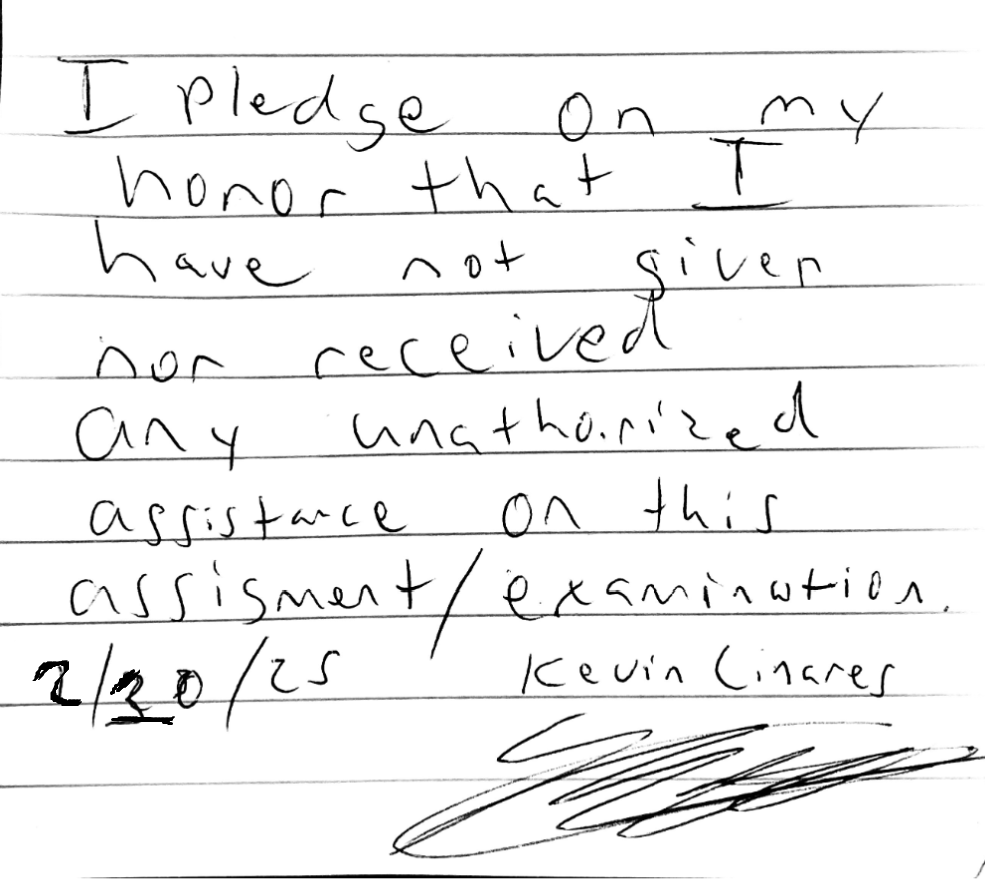
\includegraphics[width=3.03125in,height=\textheight]{honor_hw3.png}}{}}\label{section}

\begin{enumerate}
\def\labelenumi{\arabic{enumi}.}
\tightlist
\item
  The following data come from a case-control study. The cases were
  sampled from a registry of all lung cancer patients at a set of 6
  clinics. The controls were sampled from the patients at the 6 clinics
  who did not have lung cancer. Each group was asked if they had ever
  been regular smokers. The researchers made the following claims
  (1a-1f) based upon these data. State whether the claim is TRUE or
  FALSE and explain your answer. In this case, the population of
  interest is those persons who visited the 6 clinics over a specified
  time period.
\end{enumerate}

\begin{Shaded}
\begin{Highlighting}[]
\NormalTok{a }\OtherTok{\textless{}{-}} \DecValTok{126}
\NormalTok{b }\OtherTok{\textless{}{-}} \DecValTok{100} 
\NormalTok{c }\OtherTok{\textless{}{-}} \DecValTok{35}
\NormalTok{d }\OtherTok{\textless{}{-}} \DecValTok{61}

\CommentTok{\# replicated table}
\NormalTok{matrix\_ct }\OtherTok{\textless{}{-}} \FunctionTok{matrix}\NormalTok{(}
  \FunctionTok{c}\NormalTok{(a, b, c, d),}
  \AttributeTok{ncol =} \DecValTok{2}\NormalTok{, }\AttributeTok{byrow =} \ConstantTok{TRUE}\NormalTok{)}

\FunctionTok{dimnames}\NormalTok{(matrix\_ct) }\OtherTok{\textless{}{-}} \FunctionTok{list}\NormalTok{(}
  \AttributeTok{Smoker =} \FunctionTok{c}\NormalTok{(}\StringTok{"Yes"}\NormalTok{, }\StringTok{"No"}\NormalTok{),}
  \StringTok{"Lung Cancer"} \OtherTok{=} \FunctionTok{c}\NormalTok{(}\StringTok{"Yes"}\NormalTok{, }\StringTok{"No"}\NormalTok{))}

\NormalTok{matrix\_ct }
\end{Highlighting}
\end{Shaded}

\begin{verbatim}
      Lung Cancer
Smoker Yes  No
   Yes 126 100
   No   35  61
\end{verbatim}

a) The proportion with cancer in the population is estimated by
(126+35)/(126+35+100+61)=0.5.

\begin{itemize}
\tightlist
\item
  False, the proportion of the disease is the overall estimate of the
  disease in the sample from these clinics, and not the population. This
  estimate is not an un-biased estimate of the population since this is
  from a retrospective design. However, the proportion of disease
  calculation for the sample is correct.
  \(\hat{p}_{disease} = \frac{a+c}{t}\).
\end{itemize}

b) The proportion of the population that smokes is estimated by
(126+100)/ (126+35+100+61)=0.702.

\begin{itemize}
\tightlist
\item
  False, the proportion is the overall estimate of the exposure in the
  sample from these clinics, and not the population. This estimate is
  not an un-biased estimate of the population since this is from a
  retrospective design. However, the proportion of exposure calculation
  for the sample is correct. \(\hat{p}_{exposure} = \frac{a+b}{t}\).
\end{itemize}

c) The probability of having lung cancer among Smokers is estimated by
126/226=0.558.

\begin{itemize}
\tightlist
\item
  True, the probability of having the disease given the exposure, also
  known as the incidence proportion of the exposed, is given as
  \(i_{exposed} = \frac{a}{a+b} = .56\)
\end{itemize}

d) The probability of having lung cancer among Non-Smokers is estimated
by 35/96=0.365.

\begin{itemize}
\tightlist
\item
  True, the probability of not having the disease given the exposure,
  also known as the incidence proportion of the unexposed, is given as
  \(i_{unexposed} = \frac{c}{c+d} = .37\)
\end{itemize}

e) The relative risk of having lung cancer, Smokers relative to
non-Smokers is 0.558/0.365=1.529.

\begin{itemize}
\tightlist
\item
  False, the relative risk in a retrospective study cannot be calculated
  correctly, but instead using the odds ratio while making assumptions
  about the data.
\end{itemize}

f) The odds ratio of having lung cancer for smokers relative to
non-smokers is (126\emph{61)/(35}100)=2.196.

\begin{itemize}
\tightlist
\item
  True, the odds ratio is given as \(\hat{o} = \frac{ad}{bc}\), which
  corresponds with the given calculation of 2.20.
\end{itemize}

g) Now you must find the 95\% CI for the odds ratio from these data.The
odds ratio of having lung cancer for smokers relative to non-smokers is
(126\emph{61)/(35}100)=2.196.

\begin{itemize}
\tightlist
\item
  The variance for the odds ratio on the natural log is given as
  \(\hat{v}\{\ln(\hat{o}) \} = \frac{1}{a} + \frac{1}{b} + \frac{1}{c} + \frac{1}{d}\)
  while the 95\% confidence interval is given as
  \(\ln{\hat{o}} \pm 1.96 \times \sqrt{\hat{v}\{\ln(\hat{o}) \}}\).
\end{itemize}

\begin{Shaded}
\begin{Highlighting}[]
\CommentTok{\# compute OR }
\NormalTok{OR }\OtherTok{\textless{}{-}}\NormalTok{ (a}\SpecialCharTok{*}\NormalTok{d)}\SpecialCharTok{/}\NormalTok{(b}\SpecialCharTok{*}\NormalTok{c)}
\FunctionTok{print}\NormalTok{(}\FunctionTok{str\_c}\NormalTok{(}\StringTok{"Printing Odds Ratio . . . "}\NormalTok{, OR))}
\end{Highlighting}
\end{Shaded}

\begin{verbatim}
[1] "Printing Odds Ratio . . . 2.196"
\end{verbatim}

\begin{Shaded}
\begin{Highlighting}[]
\CommentTok{\# calculate variance for odds ratio}
\NormalTok{var\_OR }\OtherTok{\textless{}{-}}\NormalTok{ (}\DecValTok{1}\SpecialCharTok{/}\NormalTok{matrix\_ct[}\DecValTok{1}\NormalTok{, }\DecValTok{1}\NormalTok{]) }\SpecialCharTok{+}\NormalTok{ (}\DecValTok{1}\SpecialCharTok{/}\NormalTok{matrix\_ct[}\DecValTok{1}\NormalTok{, }\DecValTok{2}\NormalTok{]) }\SpecialCharTok{+}
\NormalTok{(}\DecValTok{1}\SpecialCharTok{/}\NormalTok{matrix\_ct[}\DecValTok{2}\NormalTok{, }\DecValTok{1}\NormalTok{]) }\SpecialCharTok{+}\NormalTok{ (}\DecValTok{1}\SpecialCharTok{/}\NormalTok{matrix\_ct[}\DecValTok{2}\NormalTok{, }\DecValTok{2}\NormalTok{])}

\CommentTok{\# calculate 95\% CI}
\NormalTok{lower }\OtherTok{\textless{}{-}} \FunctionTok{exp}\NormalTok{(}\FunctionTok{log}\NormalTok{(OR) }\SpecialCharTok{{-}} \FloatTok{1.96} \SpecialCharTok{*} \FunctionTok{sqrt}\NormalTok{(var\_OR))}
\NormalTok{upper }\OtherTok{\textless{}{-}} \FunctionTok{exp}\NormalTok{(}\FunctionTok{log}\NormalTok{(OR) }\SpecialCharTok{+} \FloatTok{1.96} \SpecialCharTok{*} \FunctionTok{sqrt}\NormalTok{(var\_OR))}
\FunctionTok{print}\NormalTok{(}\FunctionTok{str\_c}\NormalTok{(}\StringTok{"Printing 95\% CI . . . ["}\NormalTok{, lower, }\StringTok{", "}\NormalTok{, upper, }\StringTok{"]"}\NormalTok{)) }
\end{Highlighting}
\end{Shaded}

\begin{verbatim}
[1] "Printing 95% CI . . . [1.34321586157116, 3.59020179702107]"
\end{verbatim}

\begin{itemize}
\tightlist
\item
  Smokers are 2.2 {[}1.3, 3.6{]} times more likely than non-smokers to
  develop lung cancer.
\end{itemize}

\newpage

\begin{enumerate}
\def\labelenumi{\arabic{enumi}.}
\setcounter{enumi}{1}
\tightlist
\item
  The following data come from a retrospective study of the association
  between smoking and bladder cancer.
\end{enumerate}

\begin{Shaded}
\begin{Highlighting}[]
\CommentTok{\# replicated table}
\NormalTok{a }\OtherTok{\textless{}{-}} \DecValTok{250}
\NormalTok{b }\OtherTok{\textless{}{-}} \DecValTok{99750} 
\NormalTok{c }\OtherTok{\textless{}{-}} \DecValTok{125}
\NormalTok{d }\OtherTok{\textless{}{-}} \DecValTok{199875}

\NormalTok{matrix\_ct }\OtherTok{\textless{}{-}} \FunctionTok{matrix}\NormalTok{(}
  \FunctionTok{c}\NormalTok{(a, b, c, d),}
  \AttributeTok{ncol =} \DecValTok{2}\NormalTok{,}
  \AttributeTok{byrow =} \ConstantTok{TRUE}
\NormalTok{)}

\FunctionTok{dimnames}\NormalTok{(matrix\_ct) }\OtherTok{\textless{}{-}} \FunctionTok{list}\NormalTok{(}
  \AttributeTok{Smoker =} \FunctionTok{c}\NormalTok{(}\StringTok{"Yes"}\NormalTok{, }\StringTok{"No"}\NormalTok{),}
  \StringTok{"Bladder Cancer"} \OtherTok{=} \FunctionTok{c}\NormalTok{(}\StringTok{"Yes"}\NormalTok{, }\StringTok{"No"}\NormalTok{)}
\NormalTok{)}

\NormalTok{matrix\_ct}
\end{Highlighting}
\end{Shaded}

\begin{verbatim}
      Bladder Cancer
Smoker Yes     No
   Yes 250  99750
   No  125 199875
\end{verbatim}

a) Given that we cannot estimate the relative risk from these data, what
assumption do we need to make in order to estimate the attributable risk
from these data?

\begin{itemize}
\tightlist
\item
  In a retrospective design study we cannot easily estimate an unbiased
  relative risk, particularly in small samples studies. One assumption
  we can make is that the disease is rare and we can estimate the
  relative risk using the odds ratio. However, even with this rare
  disease assumption the odds ratio is not exactly equal to the relative
  risk, but rather an approximation.
\end{itemize}

b) Please estimate the attributable risk for the population of having
bladder cancer due to smoking. What is a 95\% confidence interval around
the estimated attributable risk for the population?

\begin{itemize}
\tightlist
\item
  The attributable risk in the population cannot be estimated without
  the assumption of rare disease. Here we assume that the incident rate
  for the disease is small and then we can use the odds ratio as an
  estimate of the relative risk. The attributable risk in the population
  is therefore expressed as:
\end{itemize}

\[
\hat{A_{pop}} = \frac{ad-bc}{d(a+c)}
\]

\begin{Shaded}
\begin{Highlighting}[]
\NormalTok{A\_pop }\OtherTok{\textless{}{-}}\NormalTok{ (a}\SpecialCharTok{*}\NormalTok{d }\SpecialCharTok{{-}}\NormalTok{ b}\SpecialCharTok{*}\NormalTok{c) }\SpecialCharTok{/}\NormalTok{ (d }\SpecialCharTok{*}\NormalTok{(a}\SpecialCharTok{+}\NormalTok{c)) ; A\_pop}
\end{Highlighting}
\end{Shaded}

\begin{verbatim}
[1] 0.5003127
\end{verbatim}

\begin{itemize}
\tightlist
\item
  We can proceed to calculate the variance of \(\hat{A_{pop}}\) as:
\end{itemize}

\[
V(\ln(1-\hat{A}_{pop}) =  \left[ \frac{a}{c(a+c)}+\frac{b}{d(b+d)} \right]
\]

\begin{Shaded}
\begin{Highlighting}[]
\NormalTok{V }\OtherTok{\textless{}{-}}\NormalTok{  ( (a }\SpecialCharTok{/}\NormalTok{ (c}\SpecialCharTok{*}\NormalTok{(a}\SpecialCharTok{+}\NormalTok{c))) }\SpecialCharTok{+}\NormalTok{ (b}\SpecialCharTok{/}\NormalTok{(d}\SpecialCharTok{*}\NormalTok{(b}\SpecialCharTok{+}\NormalTok{d))) ) ; V}
\end{Highlighting}
\end{Shaded}

\begin{verbatim}
[1] 0.005334999
\end{verbatim}

\begin{itemize}
\tightlist
\item
  Which we can than use to calculate our 95\% confidence intervals as:
\end{itemize}

\[
95\% \text{ C.I.} = 
1 - \exp\biggl( \ln(1-\hat{A}_{pop}) \pm 1.96 \sqrt{V\biggl(\ln(1-\hat{A}_{pop} )\biggl)} \biggr)
\]

\begin{Shaded}
\begin{Highlighting}[]
\NormalTok{LCL }\OtherTok{\textless{}{-}}  \DecValTok{1}\SpecialCharTok{{-}}\FunctionTok{exp}\NormalTok{( }\FunctionTok{log}\NormalTok{(}\DecValTok{1}\SpecialCharTok{{-}}\NormalTok{A\_pop) }\SpecialCharTok{+} \FloatTok{1.96} \SpecialCharTok{*} \FunctionTok{sqrt}\NormalTok{(V))  ; LCL}
\end{Highlighting}
\end{Shaded}

\begin{verbatim}
[1] 0.4234033
\end{verbatim}

\begin{Shaded}
\begin{Highlighting}[]
\NormalTok{UCL }\OtherTok{\textless{}{-}}  \DecValTok{1}\SpecialCharTok{{-}}\FunctionTok{exp}\NormalTok{( }\FunctionTok{log}\NormalTok{(}\DecValTok{1}\SpecialCharTok{{-}}\NormalTok{A\_pop) }\SpecialCharTok{{-}} \FloatTok{1.96} \SpecialCharTok{*} \FunctionTok{sqrt}\NormalTok{(V))  ; UCL}
\end{Highlighting}
\end{Shaded}

\begin{verbatim}
[1] 0.5669635
\end{verbatim}

\begin{itemize}
\tightlist
\item
  The attributable risk in the population in this retrospective study is
  an estimated reduction in incidence of 50\% if the whole population
  were unexposed, comparing with actual exposure. Our 95\% CI is between
  42\% and 57\%.
\end{itemize}

\newpage

\begin{enumerate}
\def\labelenumi{\arabic{enumi}.}
\setcounter{enumi}{2}
\tightlist
\item
  The following data come from a fictional prospective study of the
  association between baldness and heart disease. The sample was
  randomly selected from the population and then followed to see if they
  developed baldness and/or heart disease.
\end{enumerate}

\begin{Shaded}
\begin{Highlighting}[]
\CommentTok{\# replicated table}
\NormalTok{a }\OtherTok{\textless{}{-}} \DecValTok{127}
\NormalTok{b }\OtherTok{\textless{}{-}} \DecValTok{1224} 
\NormalTok{c }\OtherTok{\textless{}{-}} \DecValTok{548}
\NormalTok{d }\OtherTok{\textless{}{-}} \DecValTok{7611}

\NormalTok{t }\OtherTok{\textless{}{-}} \FunctionTok{sum}\NormalTok{(a, b, c, d)}

\NormalTok{matrix\_ct }\OtherTok{\textless{}{-}} \FunctionTok{matrix}\NormalTok{(}
  \FunctionTok{c}\NormalTok{(a, b, c, d),}
  \AttributeTok{ncol =} \DecValTok{2}\NormalTok{,}
  \AttributeTok{byrow =} \ConstantTok{TRUE}
\NormalTok{)}

\FunctionTok{dimnames}\NormalTok{(matrix\_ct) }\OtherTok{\textless{}{-}} \FunctionTok{list}\NormalTok{(}
  \AttributeTok{Baldness =} \FunctionTok{c}\NormalTok{(}\StringTok{"Yes"}\NormalTok{, }\StringTok{"No"}\NormalTok{),}
  \StringTok{"Heart Disease"} \OtherTok{=} \FunctionTok{c}\NormalTok{(}\StringTok{"Yes"}\NormalTok{, }\StringTok{"No"}\NormalTok{)}
\NormalTok{)}

\NormalTok{matrix\_ct}
\end{Highlighting}
\end{Shaded}

\begin{verbatim}
        Heart Disease
Baldness Yes   No
     Yes 127 1224
     No  548 7611
\end{verbatim}

a) Please graph the proportion that has heart disease in each group
(i.e.~bald and not).

\begin{Shaded}
\begin{Highlighting}[]
\CommentTok{\# calculate proportion using incidence for exposed \& unexposed}
\NormalTok{Baldness }\OtherTok{\textless{}{-}}\NormalTok{ a }\SpecialCharTok{/}\NormalTok{ (a}\SpecialCharTok{+}\NormalTok{b)}
\NormalTok{no\_Baldness }\OtherTok{\textless{}{-}}\NormalTok{ c }\SpecialCharTok{/}\NormalTok{ (c}\SpecialCharTok{+}\NormalTok{d)}

\CommentTok{\# combine proportions and plot}
\FunctionTok{as.data.frame}\NormalTok{(}\FunctionTok{rbind}\NormalTok{(Baldness, no\_Baldness)) }\SpecialCharTok{|\textgreater{}} 
  \FunctionTok{rownames\_to\_column}\NormalTok{() }\SpecialCharTok{|\textgreater{}} 
  \FunctionTok{ggplot}\NormalTok{(}\FunctionTok{aes}\NormalTok{(}\AttributeTok{x=}\NormalTok{rowname, }\AttributeTok{y=}\NormalTok{V1)) }\SpecialCharTok{+}
  \FunctionTok{geom\_col}\NormalTok{(}\AttributeTok{fill=}\StringTok{"dodgerblue"}\NormalTok{, }\AttributeTok{alpha=}\NormalTok{.}\DecValTok{7}\NormalTok{) }\SpecialCharTok{+}
\NormalTok{  ggthemes}\SpecialCharTok{::}\FunctionTok{theme\_hc}\NormalTok{() }\SpecialCharTok{+}
  \FunctionTok{labs}\NormalTok{(}\AttributeTok{title =}  \StringTok{"Heart Disease Incidents by baldness"}\NormalTok{) }\SpecialCharTok{+}
  \FunctionTok{ylab}\NormalTok{(}\StringTok{"Proportions"}\NormalTok{) }\SpecialCharTok{+}
  \FunctionTok{xlab}\NormalTok{(}\StringTok{""}\NormalTok{) }
\end{Highlighting}
\end{Shaded}

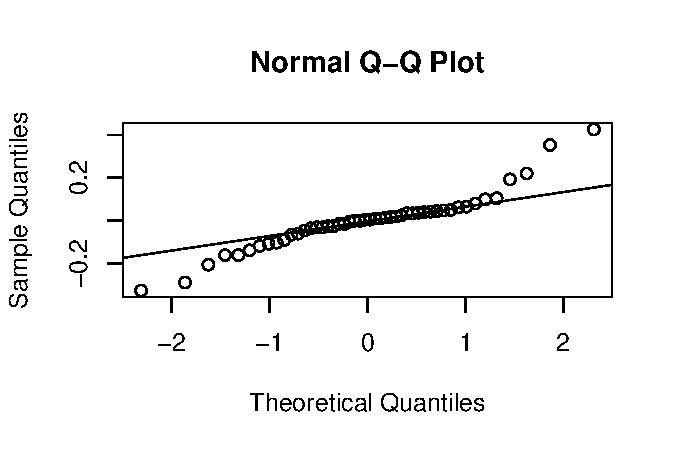
\includegraphics{HW_3_files/figure-pdf/unnamed-chunk-8-1.pdf}

b) Please estimate the attributable risk for the population of having
heart disease due to baldness. What is a 95\% confidence interval around
this estimate?

\begin{itemize}
\tightlist
\item
  For prospective studies we can estimate the attributable risk in the
  population as:
\end{itemize}

\[
\hat{A}_{pop} = \frac{ad-bc}{(a+c)(c+d)}
\]

\begin{itemize}
\tightlist
\item
  which we can than estimate the variance for \(\hat{A_{pop}}\) as:
\end{itemize}

\[
\hat{V} \bigl\{ \hat{A_{pop}}  \bigl\} = \frac{
ct \bigr[ad(t-c) + bc^2 \bigr]}
{(a+c)^3(c+d)^3}
\]

\begin{Shaded}
\begin{Highlighting}[]
\CommentTok{\# calculate attributable risk in the population}
\NormalTok{A\_pop }\OtherTok{\textless{}{-}}\NormalTok{ (a}\SpecialCharTok{*}\NormalTok{d }\SpecialCharTok{{-}}\NormalTok{ b}\SpecialCharTok{*}\NormalTok{c) }\SpecialCharTok{/}\NormalTok{ ((a}\SpecialCharTok{+}\NormalTok{c)}\SpecialCharTok{*}\NormalTok{ (c}\SpecialCharTok{+}\NormalTok{d)) ; A\_pop }\CommentTok{\# fraction}
\end{Highlighting}
\end{Shaded}

\begin{verbatim}
[1] 0.05371846
\end{verbatim}

\begin{Shaded}
\begin{Highlighting}[]
\CommentTok{\# estimate variance}

\NormalTok{V }\OtherTok{\textless{}{-}}\NormalTok{ (b }\SpecialCharTok{+}\NormalTok{ A\_pop}\SpecialCharTok{*}\NormalTok{ (a}\SpecialCharTok{+}\NormalTok{d)) }\SpecialCharTok{/}\NormalTok{ (t}\SpecialCharTok{*}\NormalTok{c) ;  V}
\end{Highlighting}
\end{Shaded}

\begin{verbatim}
[1] 0.0003146272
\end{verbatim}

\begin{itemize}
\tightlist
\item
  As before, we calculate 95\% CI.
\end{itemize}

\begin{Shaded}
\begin{Highlighting}[]
\NormalTok{LCL }\OtherTok{\textless{}{-}}  \DecValTok{1}\SpecialCharTok{{-}}\FunctionTok{exp}\NormalTok{( }\FunctionTok{log}\NormalTok{(}\DecValTok{1}\SpecialCharTok{{-}}\NormalTok{A\_pop) }\SpecialCharTok{+} \FloatTok{1.96} \SpecialCharTok{*} \FunctionTok{sqrt}\NormalTok{(V))  ; LCL}
\end{Highlighting}
\end{Shaded}

\begin{verbatim}
[1] 0.02024151
\end{verbatim}

\begin{Shaded}
\begin{Highlighting}[]
\NormalTok{UCL }\OtherTok{\textless{}{-}}  \DecValTok{1}\SpecialCharTok{{-}}\FunctionTok{exp}\NormalTok{( }\FunctionTok{log}\NormalTok{(}\DecValTok{1}\SpecialCharTok{{-}}\NormalTok{A\_pop) }\SpecialCharTok{{-}} \FloatTok{1.96} \SpecialCharTok{*} \FunctionTok{sqrt}\NormalTok{(V))  ; UCL}
\end{Highlighting}
\end{Shaded}

\begin{verbatim}
[1] 0.08605154
\end{verbatim}

\begin{itemize}
\tightlist
\item
  We estimate an attributable risk in the population of 5\% of heart
  disease due to baldness, meaning that 5\% of heart disease cases in
  the population could be prevented if baldness was eliminated, 95\% CI
  between 2\% and 9\%.
\end{itemize}




\end{document}
